\documentclass[../RelazioneFinale.tex]{subfiles}

\begin{document}

	\chapter{Architettura}
	\label{cap:Architettura}
	
		\section{Introduzione}
			Per poter gestire meglio lo sviluppo, l'intero sistema è stato suddiviso in due parti visibili concettualmente e concretizzate in \emph{solution} (soluzioni), configurazioni definite dall'ambiente di sviluppo Visual Studio. Esse sono:
			\begin{itemize}
				\item Updater Client;
				\item Updater Server.
			\end{itemize}
			Ad esse sono stati associati i vari progetti definiti all'interno dei seguenti namespace:
			\begin{description}
				\item[Updater:] racchiude le componenti principali del programma che fornisce le funzionalità di installazione e aggiornamento dei prodotti;
				\item[UIControls:] raggruppa le componenti grafiche che seguono il pattern MVVM (quindi per ogni componente grafica, view, abbiamo un corrispondente ViewModel e Model);
				\item[UpdaterClientLibrary:] contiene le componenti che incapsulano una corretta comunicazione con il servizio REST e effettuano le operazioni per scaricare, installare e aggiornare un prodotto software;
				\item[UpdaterSerialization:] contiene le componenti che racchiudono i dati trasmessi tra server e client, quindi serializzati.
				\item[UpdaterServer:] contiene le componenti necessarie per il funzionamento del servizio RESTful;
				\item[UpdaterDBEF:] (DBEF = DataBase Entity Framework) contiene le componenti che implementano la tecnica ORM la quale consente una facile relazione tra le componenti orientate agli oggetti e il database relazionale.
 			\end{description}
 			Di seguito l'associazione delle varie macro componenti con le \emph{solution}:
 			\begin{description}
 				\item[Updater Client] composto dalle macro componenti:
 				
 				\begin{itemize}
 					\item Updater;
 					\item UpdaterUIControls;
 					\item UpdaterClientLibrary;
 					\item UpdaterSerialization.
 				\end{itemize}
 				\item[Updater Server] composto dalle macro componenti:
 				
 				\begin{itemize}
 					\item UpdaterSerialization;
 					\item UpdaterServer;
 					\item UpdaterDBEF.
 				\end{itemize}
 			\end{description}
 			Come è possibile notare, le componenti in UpdaterSerialization sono condivise in entrambe le \emph{solution} ciò perché esse permettono lo scambio di informazioni tra client e server.
 			
 			%Sono inoltre presenti delle pagine web che consentono di svolgere le operazioni chiave nel database attraverso l'uso di un'interfaccia semplificata ossia form su pagine HTML5.
		
		\section{Architettura generale}
			L'intero sistema segue una struttura a livelli (figura \ref{fig:DipendenzeComponenti}) in cui la dipendenza tra le macro componenti segue un flusso verso il basso.
			
			\subsection*{Comunicazione tra componenti}
			La comunicazione avviene principalmente solo tra macro componenti vicine. In particolare la macro componente Updater Client Library rende indipendente le altre componenti client dalla comunicazione attraverso la rete e l'uso delle richieste HyperText Transfer Protocol (HTTP) (figura \ref{fig:UpdaterRequest}). 
			
			\subsection*{Architettura - Parte client}
			Per la parte client si è seguito il pattern Model View ViewModel (MVVM) incoraggiato dalla tecnologia WPF e rafforzato dall'uso del framework di supporto Catel. Quest'ultimo mette a disposizione tag, attributi e classi che permettono una gestione più semplice delle tre parti: View, ViewModel e Model.
			Ogni componente grafico avrà il suo corrispettivo ViewModel (logica e dati utili al componente View) e se necessario anche il Model (se in possesso di dati persistenti, per esempio prelevati dal database).
			
			\subsection*{Architettura - Parte server}
			Per la parte server invece si utilizza il framework ASP.NET il quale attraverso la definizione di classi \textbf{controller} permette la costruzione di un servizio RESTful. La comunicazione tra Web API e database avviene grazie ad Entity Framework il quale implementa la tecnica di programmazione Object-Relational Mapping (ORM).

			\vfill			
			
			\begin{figure}[h]
				\centering
				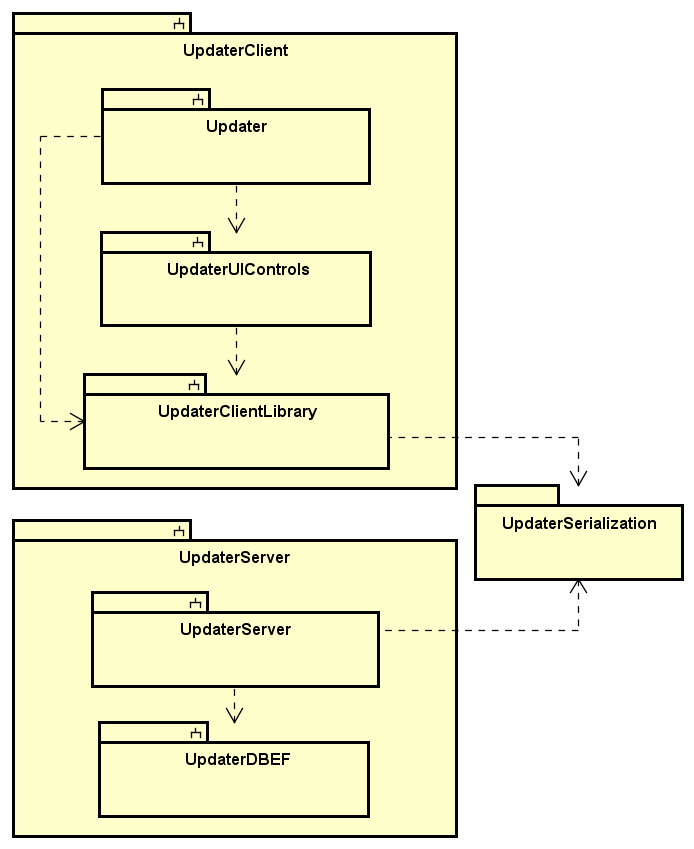
\includegraphics[scale=0.68]{DipendenzeComponenti}
				\caption{Dipendenze tra macro componenti del sistema Updater}
				\label{fig:DipendenzeComponenti}
			\end{figure}
			
			\begin{figure}[p]
				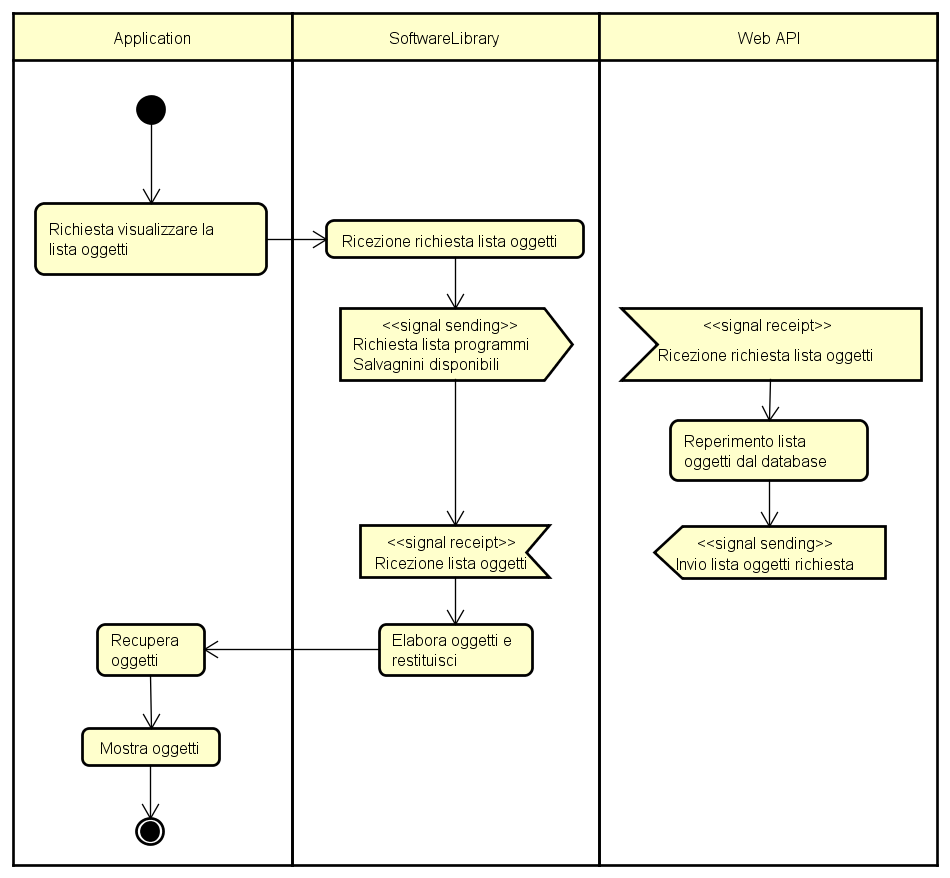
\includegraphics[width=\textwidth]{UpdaterRequest}
				\caption{Esempio generico di comunicazione tra parte client e parte server}
				\label{fig:UpdaterRequest}
			\end{figure}
		
\newpage
		
	\section{Macro componenti}
		Nella presente sezione vengono descritte in dettaglio le macro componenti riportando per ciascuna una descrizione esauriente e la struttura con le componenti interne e le relazioni tra esse. Dove necessario vengono discusse le scelte e le possibili criticità cercando di proporre soluzioni migliori e migliorie che in futuro potrebbero essere implementate.
			
			
		
		\subsection{Updater}
		
			\subsubsection{Descrizione}
				Identifica un programma eseguibile lato client composto principalmente da un'interfaccia grafica per agevolare l'utente nel download, nell'installazione o nell'aggiornamento dei prodotti software e relativi prerequisiti.
			
			\subsubsection{Responsabilità}
				\begin{itemize}
					\item Gestire l'avvio dell'applicazione WPF;
					\item Gestire eventuali parametri all'avvio dell'applicazione;
					\item Gestire la finestra principale dell'applicazione;
					\item Gestire la finestra delle impostazioni dell'applicazione;
					\item Gestire l'icona di notifica nella \emph{TaskBar}.
				\end{itemize}
			
			\subsubsection{Implementazione}

				\paragraph{Dipendenze esterne}
					\begin{itemize}
						\item WPF;
						\item Catel;
						\item MahApps;
						\item Command Line Parser.
					\end{itemize}
					
				\paragraph{Dipendenze interne}
					\begin{itemize}
						\item Salvagnini.UICatelControls;
						\item Salvagnini.UIControls.
					\end{itemize}		
			
				\paragraph{}
				Il programma si basa sul framework Windows Presentation Foundation il quale mette a disposizione la classe \verb|Application| singleton e primo oggetto istanziato all'esecuzione del programma. \verb|Application| è quindi stata ereditata dalla classe \verb|App| la quale è responsabile di:
				\begin{itemize}
					\item creare la finestra principale e la schermata secondaria delle impostazioni utente;
					\item creare la Notify Icon che comparirà nella barra dello start (\emph{TaskBar}) e della comparsa;
					\item creare avvisi (\emph{baloon}) in risposta al completamento corretto o in errore delle operazioni automatiche.
				\end{itemize}
				
				La finestra principale è identificata dalla classe \verb|MainWindows|, estende la classe \verb|MetroWindow| distribuita dall'UI toolkit \emph{MahApp} il quale applica alla finestra lo stile delle moderne applicazioni windows aderenti al design \emph{Metro}.
				Una finestra secondaria è rappresentata dalla classe \verb|SettingsView| la quale si occupa di gestire le componenti grafiche per le preferenze utente dell'intera applicazione, tali preferenze (o impostazioni) impatteranno nel funzionamento della \verb|TaskBarIcon|.				
				In se il progetto è costituito solo dalla finestra principale e dalla gestione dell'icona nella taskbar del sistema. Esso contiene prettamente componenti grafiche e la logica di base di esse e dell'avvio dell'applicazione (implicito grazie all'uso di \verb|Application|).
			
			\subsubsection{Funzionamento}
				La struttura segue il pattern MVVM come si vede in figura \ref{fig:Updater}.
				\verb|App| è una classe singleton e la prima ad essere istanziata dal framework WPF, da questa il programma inizializza la \verb|MainWindow| e tutte le componenti grafiche (View) coinvolte insieme ai rispettivi ViewModel e Model.
				Le classi interne al namespace \verb|Views| sono costituite da una parte descritta in XAML (descrive l'aspetto prettamente grafico) e una in \Csharp\ (il \emph{code behind}).
				La classe \verb|Options| usufruisce della classe \verb|IParserState| della libreria \emph{Command Line Parser} consentendo all'applicazione di essere eseguita con alcuni parametri utili per gli eventuali riavvi necessari nell'installazione di qualche prodotto software.
			
			\subsubsection{Criticità e possibili miglioramenti}
				Il pattern architetturale MVVM garantisce una certa separazione tra le componenti e l'uso del framework Catel rende le comunicazioni tra View e ViewModel molto chiare e semplici, anche tra diversi ViewModel grazie all'attributo \verb|[InterestedIn]|.
				L'uso della \emph{TaskBarIcon} costringe all'inserimento di codice di logica (e quindi non riguardante la grafica) nel \emph{code behind} della classe \verb|App| ciò oltre a non essere buona pratica dà una nuova responsabilità di più basso livello (creazione dei \emph{baloon}) rispetto alla creazione delle finestre della classe \verb|App|\footnote{\cite{beck2008implementation} Responsabilità di diverso livello rompono il \emph{principio di simmetria} individuato da Kent Beck in \emph{Implementation Pattern, cap. 3, pag. 15}.}.
				
				Nel caso in cui ci sia la necessità di aggiungere nuove responsabilità per la classe \verb|App| è necessario un redesign per spostare il codice che coinvolge la classe \verb|TaskBarIcon| ad una nuova classe. 		
			\vfill
			%\subsubsection{Struttura del package}
			\begin{figure}[h]
				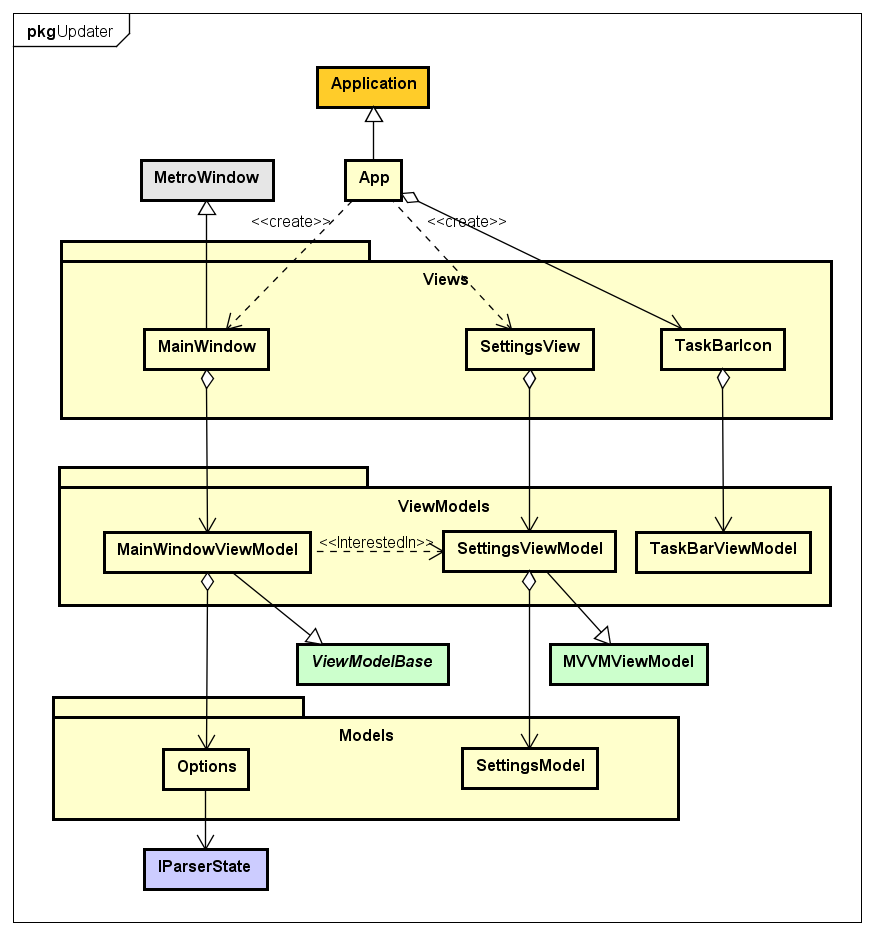
\includegraphics[width=\textwidth]{Updater}
				\label{fig:Updater}
				\caption{Struttura macro componente Updater}
			\end{figure}
				
\newpage
			
		\subsection{Updater User Interface Controls}

			\subsubsection{Descrizione}
				Identifica un insieme di componenti grafici utilizzabili da software esterno per costruire un'interfaccia grafica. Tali componenti sono utilizzate da Updater e potranno essere utilizzate da altri prodotti software.
				
			\subsubsection{Responsabilità}
			\begin{itemize}
				\item Fornire le componenti grafiche principali che consentono all'utente di visualizzare, scaricare, installare, reinstallare e aggiornare un prodotto software.
			\end{itemize}
			
			\subsubsection{Implementazione}
			
				\paragraph{Dipendenze esterne}
					\begin{itemize}
						\item WPF;
						\item Catel;
						\item MahApps.
					\end{itemize}
				
				\paragraph{Dipendenze interne}
					\begin{itemize}
						\item Salvagnini.UICatelControls;
						\item Salvagnini.UIControls.
					\end{itemize}
					
				\paragraph{}							
			La macro componente è costituita da tre elementi grafici principali: 
			\begin{enumerate}
				\item ProductsPanel;
				\item ProductControl;
				\item ProductInfo.
			\end{enumerate}
			
			Il primo rappresenta una lista degli elementi grafici \verb|ProductControl| e offre vari filtri da applicare ad essa compresa una ricerca per nome.
			Il secondo rappresenta un singolo prodotto software e fornisce i pulsanti per effettuare le operazioni di installazione, reinstallazione, download e aggiornamento.
			Il terzo è legato al primo con l'attributo offerto da Catel \verb|[InterestedIn]|, in base alla selezione di un elemento della lista questo mostra informazioni più dettagliate su di esso.
			Tutti gli elementi implementano il pattern MVVM pertanto sono scomposti in tre parti. La parte prettamente visiva (\emph{View}) è costruita in XAML e \Csharp\ mentre le altre in puro \Csharp.
						
			\subsubsection{Funzionamento}
				WPF instanzia le classi \verb|View|. \verb|ProductInfoView| istanzia il proprio \verb|Model|, ossia \verb|ProductInfoViewModel|.
				
				Per \verb|ProductsPanelView| invece il comportamento è diverso (figura \ref{fig:CreationUIControls}), Se il proprio \verb|ProductsPanelViewModel| non è già istanziato prima costruisce \verb|ProductsPanelModel|, poi \verb|ProductsPanelViewModel|. Dopo la creazione di \verb|ProductsPanelModel|, \verb|ProductsPanelViewModel| incarica \verb|ProductsPanelModel| di eseguire una richiesta HTTP per recuperare le informazioni sui prodotti software.
				
				Viene quindi istanziato un \verb|ProductControlModel| per ogni prodotto software. Terminata questa operazione, \verb|ProductsPanelViewModel| può istanziare per ogni \verb|ProductControlModel| un rispettivo \verb|ProductControlViewModel|.
				Infine grazie al meccanismo del \verb|DataContext| di WPF la classe \verb|ProductControlView| può recuperare il rispettivo \verb|ProductControlViewModel|.
				
			\begin{figure}[h]
				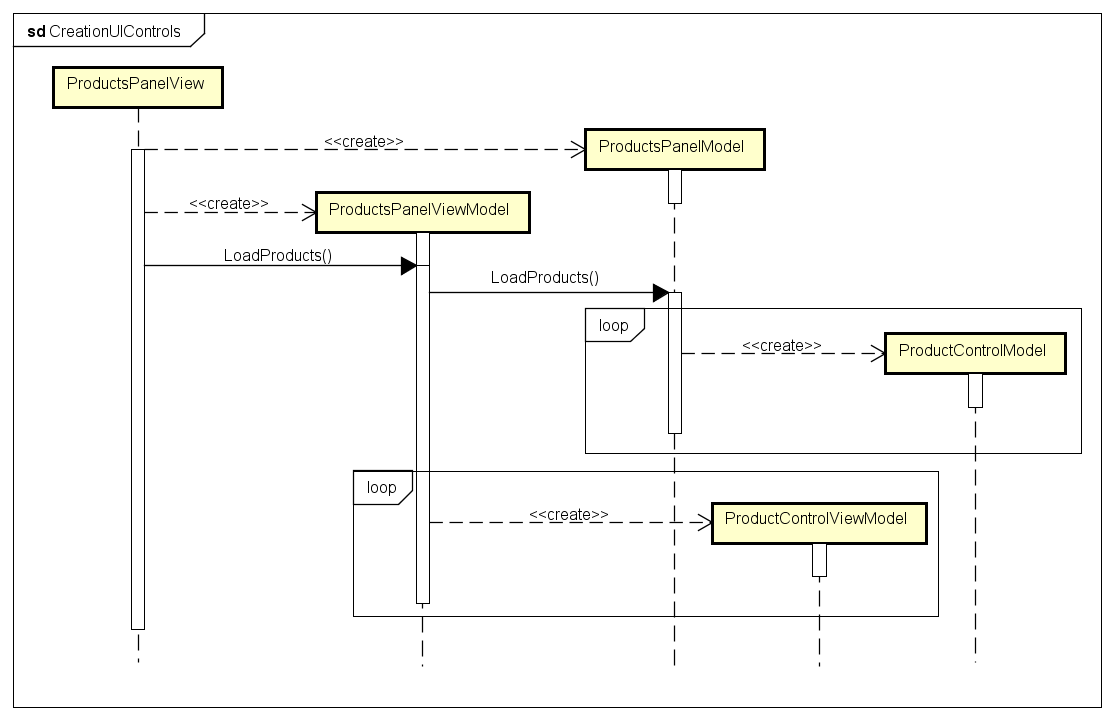
\includegraphics[width=\textwidth]{CreationUIControls}
				\label{fig:CreationUIControls}
				\caption{Diagramma di sequenza per la costruzione degli elementi grafici UIControls}
			\end{figure}
			
			\subsubsection{Criticità e possibili miglioramenti}
				Il macro componente presenta confusione nell'uso di \verb|DataContext|, inoltre le responsabilità sono confuse con il risultato di un necessario redesign. Infatti prima vengono costruito i vari \verb|ProductControlModel| e in seguito i \verb|ProductControlViewModel| mancando di coesione e incrementando la complessità della struttura. Tutto ciò rende ancor più difficile la comprensione delle componenti e quindi la modifica futura.
				
				La classe \verb|ProductControlModel| racchiude in sé logica delle componenti di \emph{Updater Client Library} poiché all'interno di queste operazioni sono necessari dei feedback che impattano nell'interfaccia grafica, inoltre è possibile che durante l'operazione sia richiesto il riavvio dell'app. Un'alternativa forse più valida sposterebbe la logica nella libreria definendo la possibilità che essa lanci degli eventi indicanti lo stato delle operazioni e a questi \verb|ProductControlModel| reagisca opportunamente. Questa alternativa non è stata implementata per evitare la complessità nella gestione della concorrenza. Procedendo così infatti si verrebbe a creare una situazione in cui due differenti thread devono comunicare tra di loro.

			\vfill						
			%\subsubsection{Struttura del package}
			\begin{figure}[h]
				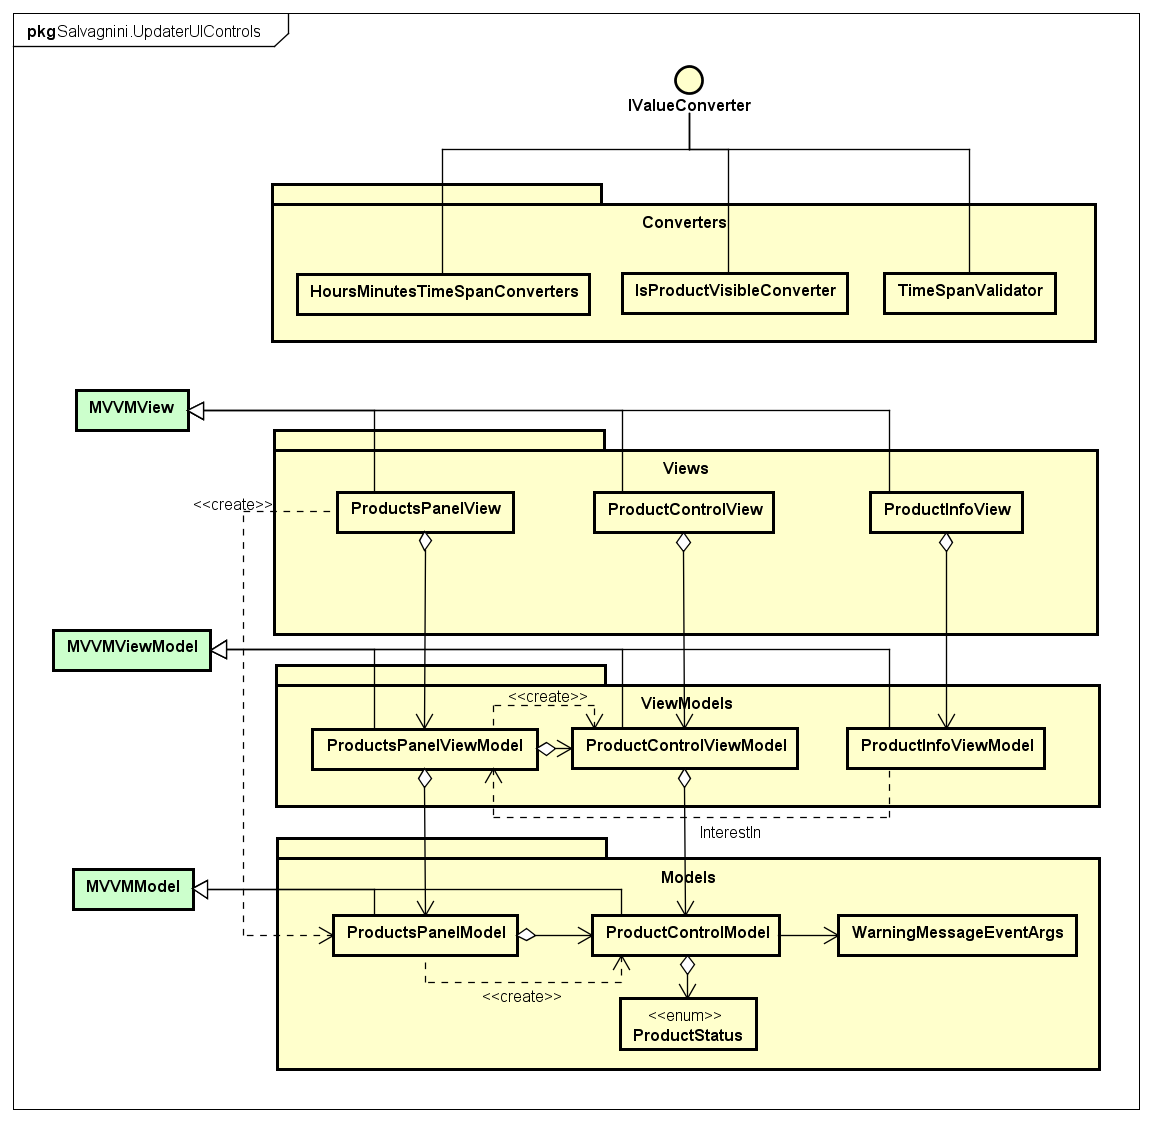
\includegraphics[width=\textwidth]{UpdaterUIControls}
				\label{fig:UpdaterUIControls}
				\caption{Struttura macro componente Updater UIControls}
			\end{figure}

\newpage
	
		\subsection{Updater Client Library}
		
			\subsubsection{Descrizione}
				Identifica un insieme di componenti software incaricate di effettuare delle operazioni di controllo locali (per es. controllare la presenza dei programmi Salvagnini) e di gestire le comunicazioni con la Web API tramite servizio REST e il formato dati JSON. Tali componenti sono utilizzate dalle macro componenti \emph{Updater} e \emph{UpdaterUIControls}.
			Le componenti sono state rese indipendenti con lo scopo di poterle riutilizzare in altri prodotti software.
			
			\subsubsection{Responsabilità}
				\begin{itemize}
					\item Incapsulare la comunicazione con il servizio REST;
					\item Consentire di effettuare su un prodotto software le seguenti operazioni:
					\begin{itemize}
						\item Download;
						\item Installazione;
						\item Reinstallazione;
						\item Aggiornamento;
					\end{itemize}
					\item Consentire l'esecuzione automatica delle operazioni elencate precedentemente;
					\item Fornire gli strumenti per il corretto riavvio dell'applicazione;
					\item Fornire gli strumenti per il salvataggio su file XML delle operazioni effettuate (per es. salvare la data di installazione di un prodotto).
				\end{itemize}
			
			\subsubsection{Implementazione}
			
				\paragraph{Dipendenze esterne}
					\begin{itemize}
						\item Catel.
					\end{itemize}
				
				\paragraph{Dipendenze interne}
					\begin{itemize}
						\item Updater Serialization.
					\end{itemize}
				
				\paragraph{}
					La libreria è costituita principalmente da tre parti:
					\begin{enumerate}
						\item Dalle componenti che si occupano di comunicare con il servizio REST e di effettuare le operazioni sui prodotti software;
						\item Dalle componenti necessarie al salvataggio di dati in formato XML;
						\item Dalle componenti che si occupano di automatizzare le operazioni;
					\end{enumerate}
					
					La prima parte è costituita da \verb|ProductWrapper| e \verb|PrerequisiteWrapper| le quali rappresentano un'incapsulazione dei dati deserializzati ricevuti dal servizio REST grazie alla classe \verb|UpdaterService|.
					Le componenti \verb|Wrapper| incapsulano tutte le operazioni che è possibile effettuare su un prodotto software e sui prerequisiti software.
					La seconda parte è costituita dalle classi all'interno del namespace \verb|Models|. La classe singleton \verb|ObjectManager| è incaricata di gestire il caricamento e il salvataggio dei dati resi persistenti in un file XML. Questi sono rappresentanti dalle classi \verb|Set| che racchiudono una struttura dati contenente oggetti contenenti i dati effettivi da salvare.
					
					La terza parte è costituita da una gerarchia, le classi concrete di tale gerarchia sono incaricate di lanciare le corrette operazioni automatiche di download, installazione o aggiornamento. Questo sulla base delle preferenze impostate dall'utente e attraverso l'uso di timer. La classe \verb|AppRestarter| racchiude la logica per il corretto riavvio dell'applicazione nel caso un'operazione automatica lo richiedesse.
											
				
			
			\subsubsection{Funzionamento}
				La libreria mette a disposizioni delle classi involucro, \verb|ProductWrapper| e \verb|PrerequisiteWrapper|, che consentono di effettuare le operazioni sui prodotti software.
				Queste stesse classi \verb|Wrapper| si occupano di rendere persistenti i dati delle operazioni svolte attraverso l'uso delle componenti interne al namespace \verb|Models|.
				Oltre alle classi \verb|Wrapper| la libreria mette a disposizione le classi \verb|AutomaticUpdates|, esse basano il proprio funzionamento in base ad un timer interno, alla loro creazione il timer parte e allo scadere la classe effettuerà l'operazione per cui è incaricata in modo completamente automatico (da qui la dipendenza tra \verb|AutomaticUpdatesController| e \verb|ProductWrapper|), il timer quindi riparte. Ogni qual volta il timer scade le classi \verb|AutomaticUpdates| lanciano un evento \verb|ProductToUpdateEventArgs| in questo modo sfruttando il pattern Observer\footnote{\cite{gamma1994design} Gang of Four. Design Patterns: Elements of Reusable Object-Oriented Software, cap. 5, pag. 326.} insito nel linguaggio \Csharp\ è possibile reagire allo scadere del timer anche in componenti esterne.
			
			\subsubsection{Criticità e possibili miglioramenti}
				Dipendenza circolare con \verb|ProductWrapper| e \verb|UpdateService|, a causa della scelta della \emph{lazy initialization} per i \verb|PrerequisiteWrapper|.
				\verb|UpdaterService| potrebbe contenere metodi statici per risolvere oppure la \emph{lazy initialization} potrebbe essere eliminata per rimuove la dipendenza.
				Manca qualche namespace che organizzerebbe meglio la libreria, ad esempio \verb|AutomaticUpdates| potrebbe essere un nuovo namespace per la gerarchia di classi strettamente connesse.
				\verb|ProductWrapper| contiene codice duplicato con \verb|AppRestarter| come conseguenza di un refactoring, oltre ad assumersi un numero elevato di responsabilità che suggerisce di spezzare la classe in più classi. La scelta di contenere tutti in una è data dal fatto che le operazioni necessarie erano ben definite (download, install e update) e si suppone che in futuro non ne servano altre. Nel caso contrario si potrebbe pensare a rappresentare ogni operazione come una classe implementando così il Command pattern\footnote{\cite{gamma1994design} Gang of Four. Design Patterns: Elements of Reusable Object-Oriented Software, cap. 5, pag. 263.}.
				
				Le componenti incaricate della deserializzazione e serializzazione dal file XML sono spesso ridondanti, l'uso di classi generiche consentirebbe un'ulteriore flessibilità al sistema evitando di dover ad ogni aggiunta di dati da rendere persistenti la codifica di ulteriori classi praticamente identiche. L'uso di classi generiche consentirebbe anche al singleton \verb|ObjectsManager| di acquisire maggior flessibilità. Attualmente questa operazione non è stata fatta per limiti tecnologici e conoscitivi del framework Catel, si è sperimentato infatti che non è possibile rendere generica una classe che estende \verb|ModelBase|, probabilmente il limite deriva dal fatto che i tipi parametrici contano solo nella precompilazione, di fatto poi tutto è tipizzato con la classe \verb|Object| di \Csharp\, in questo modo il meccanismo di serializzazione non può più distinguere una classe generica istanziata con un tipo da un'altra istanziata con tipo diverso.
				
							
			%\subsubsection{Struttura del package}
			\begin{figure}[p]
				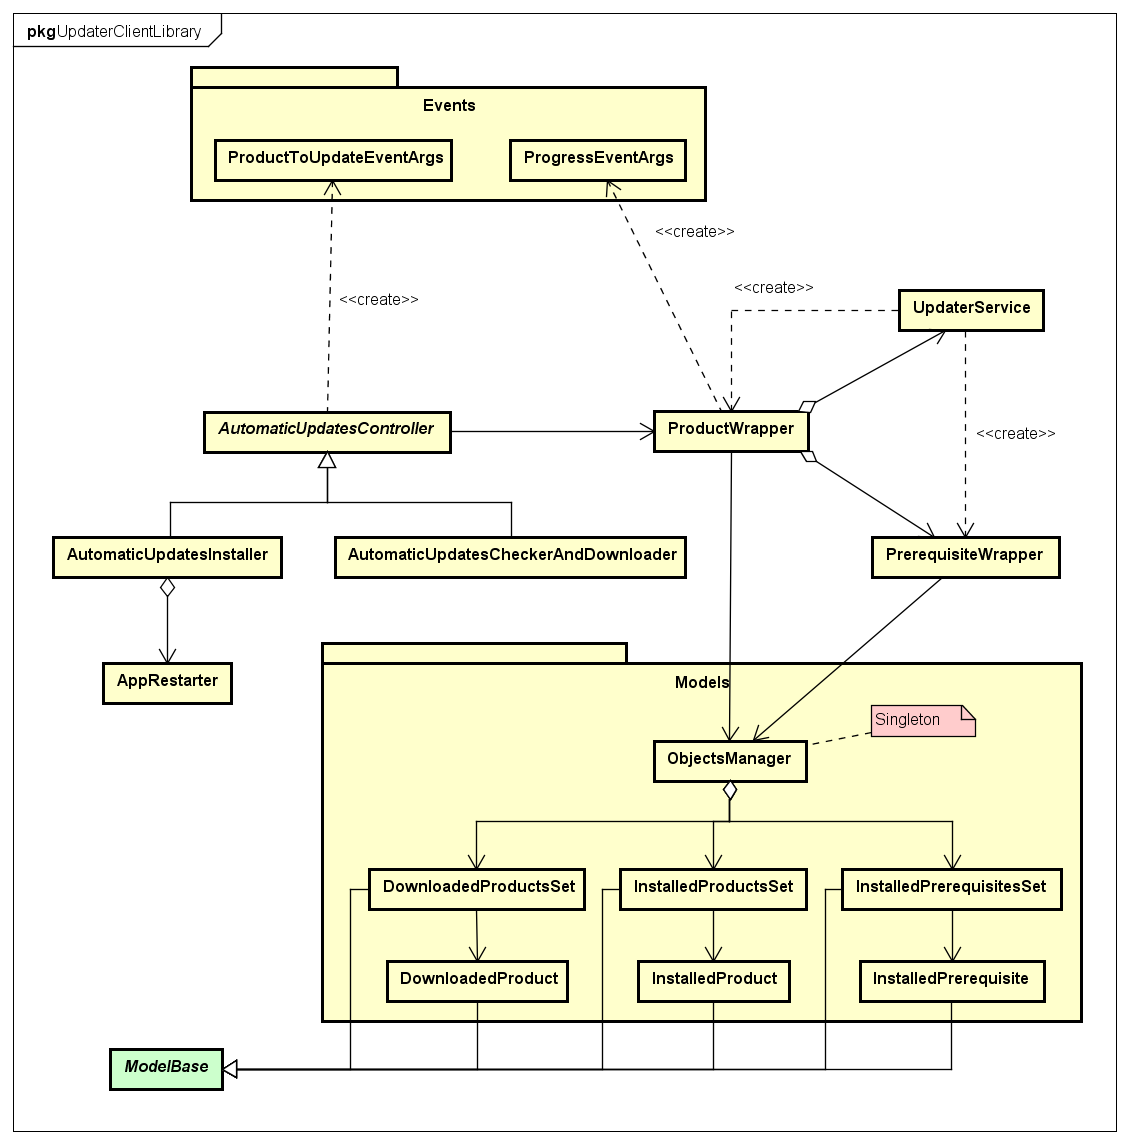
\includegraphics[width=\textwidth]{UpdaterClientLibrary}
				\label{fig:UpdaterClientLibrary}
				\caption{Struttura macro componente Updater Client Library}
			\end{figure}
		
\newpage
		
		\subsection{Updater Serialization}
		
			\subsubsection{Descrizione}
				Identifica l'insieme di definizioni di oggetti che permettono la trasmissione di dati in una rete tra server e client tramite serializzazione.
			
			\subsubsection{Responsabilità}
				\begin{itemize}
					\item Definire oggetti serializzabili contenenti dati.
				\end{itemize}
			
			\subsubsection{Implementazione}
			
				\paragraph{Dipendenze esterne} \ \par
					Nessuna.
				
				\paragraph{Dipendenze interne} \ \par
					Nessuna.
				
				\paragraph{}
				Le classi che terminano con il suffisso \verb|Object| sono definizioni di oggetti che contengono solo campi dati e costruttori. I campi dati sono etichettati con l'attributo \verb|[DataMember]| in tal modo il framework .NET è capace di trasformarle in formato JSON così da poter trasmettere informazioni attraverso una rete.
				La classe \verb|Serializer| si occupa di facilitare tale serializzazione attraverso la definizione di metodi statici per la lettura e scrittura di dati serializzati.
			
			\subsubsection{Funzionamento}
				L'unica classe del namespace che racchiude logica è \verb|Serializer|, la quale semplicemente semplifica la serializzazione e la deserializzazione definendo due metodi statici.
				Le altre componenti non racchiudono logica al loro interno.
				Nessuna componente ha dipendenze esterne per questo motivo si omette il diagramma della struttura del macro componente. 
			
			\subsubsection{Criticità e possibili miglioramenti}
				L'unico punto critico sono i costruttori delle classi \verb|Object| serializzabili. Nel caso infatti si dovesse aggiungere un campo dati si è costretti a definire un nuovo costruttore e definire un valore di default per il campo dati aggiunto. Nel caso questo non possa avvenire, tutte le dipendenze verso la classe necessiterebbero di essere modificate. Per far sì che questo sforzo di modifiche sia limitato le dipendenze verso questo macro componente sono \textbf{esclusivamente} delle macro componenti \emph{Updater Client Libary} e \emph{Updater Server} e così dovrebbe essere mantenuto in future estensioni.
		
\newpage
		
		\subsection{Updater Server}

			\subsubsection{Descrizione}
				Identifica il server con sistema IIS su cui opera la web API supportata da un database relazionale che implementerà un servizio REST col quale comunicheranno il macro componente \emph{Updater Client Library} e le pagine web amministrative del database).
			
			\subsubsection{Responsabilità}
				\begin{itemize}
					\item Fornire un servizio REST per trasmettere i dati dei prodotti software e dei relativi prerequisiti software prelevati da un database;
					\item Fornire delle pagine web amministrative per facilitare le modifiche ai dati contenuti nel database.
				\end{itemize}
			
			\subsubsection{Implementazione}
			
				\paragraph{Dipendenze esterne}
					\begin{itemize}
						\item ASP.NET;
						\item JQuery;
						\item Bootstrap;
						\item KnockoutJS.
					\end{itemize}
				
				\paragraph{Dipendenze interne}
					\begin{itemize}
						\item Updater Serialization;
						\item Updater Entity Framework Database (EFDB).
					\end{itemize}
				
				%\paragraph{Design pattern}
					%Il macro componente è stato sviluppato seguendo la struttura imposta dal framework ASP.NET.
				
				\paragraph{}
					Per la parte server del servizio REST è stata impostata la configurazione del servizio nelle componenti del namespace \verb|App_Start| preconfigurate dal framework e per richiedere l'autenticazione alle richieste HTTP è stata creata la classe \verb|BasicAuthenticationHandler|. Le componenti principali sviluppate sono le classi \verb|Controller| ossia classi i cui metodi vengono invocati in base alla richiesta HTTP ricevuta. Le gerarchie \verb|Putter| e \verb|Poster| sono state sviluppate con lo scopo di supportare tali metodi.
					Il namespace \verb|SerializableFactory| racchiude classi \verb|Factory|\footnote{\cite{gamma1994design} Gang of Four. Design Patterns: Elements of Reusable Object-Oriented Software, cap. 5, pag. 326.} le quali racchiudono metodi statici per la creazione di oggetti \verb|Object| definiti in \emph{Updater Serialization} a partire dagli oggetti distribuiti da \emph{UpdaterDBEF}.
					Per quanto riguarda la parte web (omessa nel diagramma in figura \ref{fig:UpdaterServer}) sono state create quattro pagine web in HTML5 decorate con l'aiuto del framework Bootstrap. Le pagine web interagiscono con il servizio REST tramite l'uso della tecnica Asynchronous JavaScript and XML (AJAX) resa disponibile dalla libreria JQuery (per approfondimento si veda la sezione \ref{sec:SitoWeb}). 
			
			\subsubsection{Funzionamento}
				Una volta avviata la web api vengono caricate le dovute impostazioni codificate nelle classi all'interno di \verb|App_Start|. A questo punto ad ogni richiesta http inviata al server agisce la classe \verb|BasicAuthenticationHandler| che verifica la presenza di nome utente e password corretti nella richiesta.
				Una volta accertata la richiesta il flusso del programma è passato alle classi \verb|Controller|, qui viene eseguito il codice del metodo che corrisponde all'uri della richiesta.
		
			
			\subsubsection{Criticità e possibili miglioramenti}
				Attualmente molti dati e informazioni di configurazione sono codificati direttamente mentre sarebbe molto più opportuno leggerli da file esterni garantendo così una maggiore flessibilità dell'intero sistema.
				
			%\subsubsection{Struttura del package}
			\begin{figure}[p]
				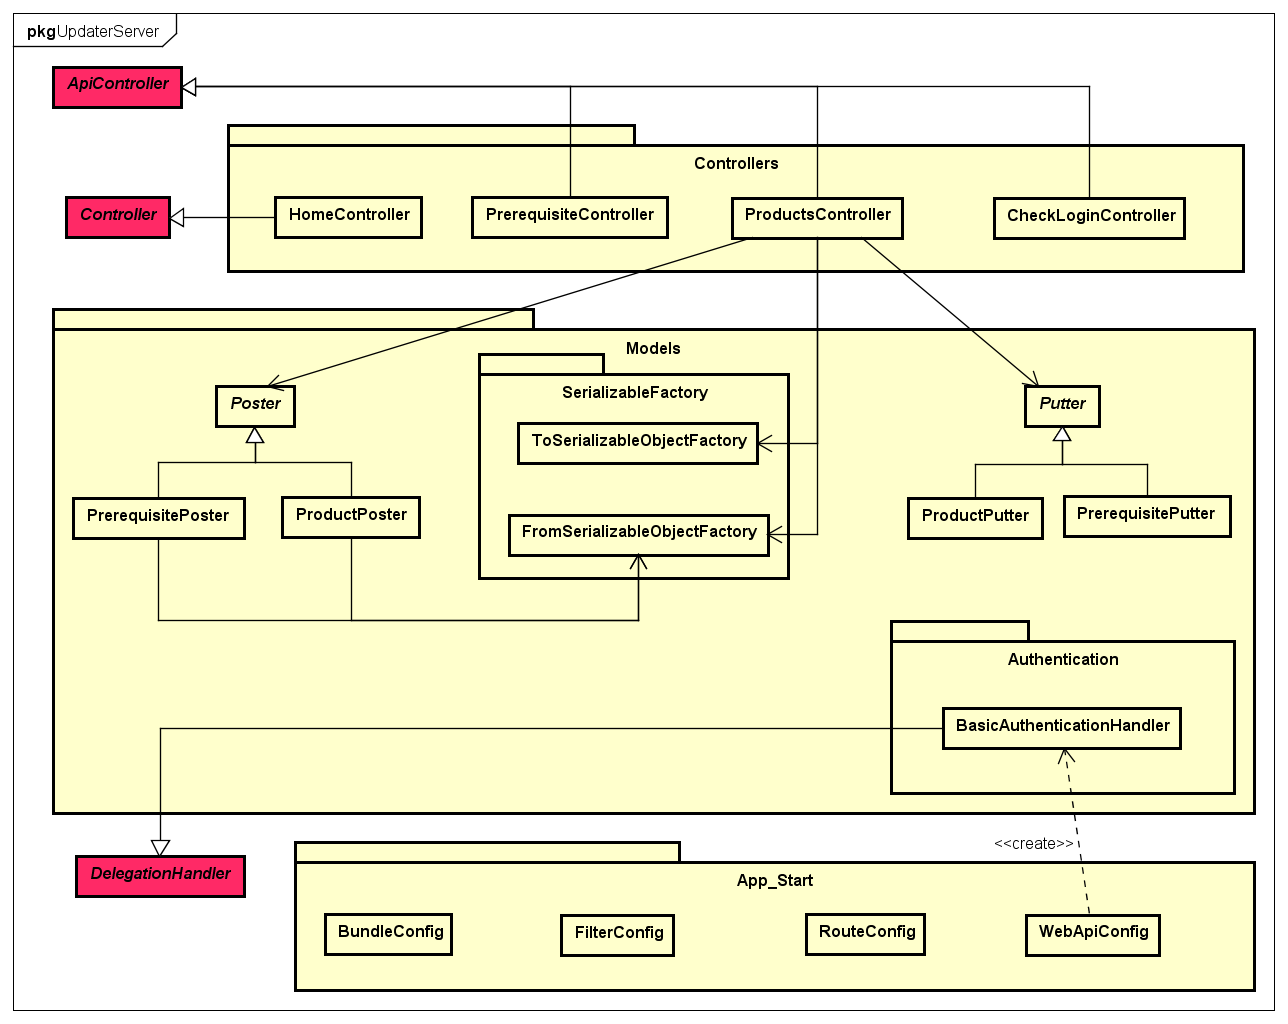
\includegraphics[width=\textwidth]{UpdaterServer}
				\label{fig:UpdaterServer}
				\caption{Struttura macro componente Updater Server}
			\end{figure}
		
\newpage
		
		\subsection{Updater Database Entity Framework (DBEF)}
		
			\subsubsection{Descrizione}
				Identifica un'insieme di componenti incaricate di mettere in relazione il paradigma della programmazione orientata agli oggetti e la base di dati relazionale.
			
			\subsubsection{Responsabilità}
				\begin{itemize}
					\item Fornire un accesso facile e semplice alla base di dati relazionale.
				\end{itemize}
			
			\subsubsection{Implementazione}
			
				\paragraph{Dipendenze esterne}
					\begin{itemize}
						\item Devart;
						\item Entity Framework.
					\end{itemize}
				
				\paragraph{Dipendenze interne} \ \par
					Nessuna.
				
				%\paragraph{Design pattern}
					%Entity Framework segue il pattern ORM.
				
				\paragraph{}
					L'utilizzo della tecnologia \emph{Devart} ha permesso di costruire le componenti strutturate su Entity Framework in modo completamente automatico a partire dal modello SQL della base di dati.
			
			\subsubsection{Funzionamento}
				Le componenti create dalla tecnologia \emph{Devart} consentono di usare la tecnologia Linq di .NET per poter usufruire attraverso programmazione funzionale di tutto il contenuto del database attraverso un'automatica conversione in oggetti.
			
			%\subsubsection{Struttura del package}
			
			\subsubsection{Criticità e possibili miglioramenti}
				Le criticità che potrebbero emergere sono principalmente le problematiche derivanti dall'uso della tecnica ORM, colpevolizzata di non rispettare i principi della programmazione ad oggetti\footnote{\url{http://www.yegor256.com/2014/12/01/orm-offensive-anti-pattern.html} \\ \url{http://seldo.com/weblog/2011/08/11/orm_is_an_antipattern}.}.
				I vantaggi però del suo uso sono stati evidenti durante lo sviluppo. La tecnologia \emph{Devart} permetteva l'aggiornamento in pochissimi passi a qualsiasi modifica nel modello della base di dati. L'uso di Entity Framework permette l'uso di Linq e quindi di accedere con una facilità disarmante ai dati nel database attraverso la programmazione funzionale e quindi codificando spesso una singola linea di codice.
				
			
\newpage		
		
	\section{Relazioni esterne tra componenti}
		Nella presente sezione vengono mostrate le relazioni esterne tra le componenti delle macro componenti attraverso l'uso di diagrammi delle classi.
			
		\subsection{Relazioni Updater}
			\begin{figure}[h]
				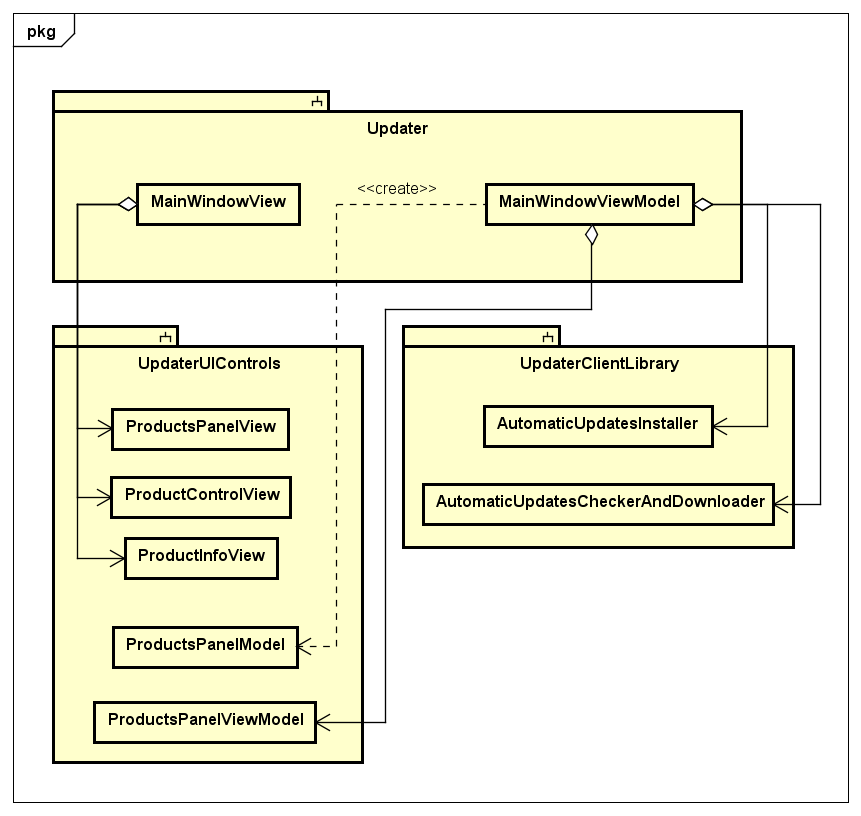
\includegraphics[width=\textwidth]{RelazioniUpdater}
				\label{fig:RelazioniUpdater}
				\caption{Relazioni componenti di Updater con le componenti di UIControls e Client Library}
			\end{figure}
			
\newpage
		\subsection{Relazioni Updater UIControls}
			\begin{figure}[h]
				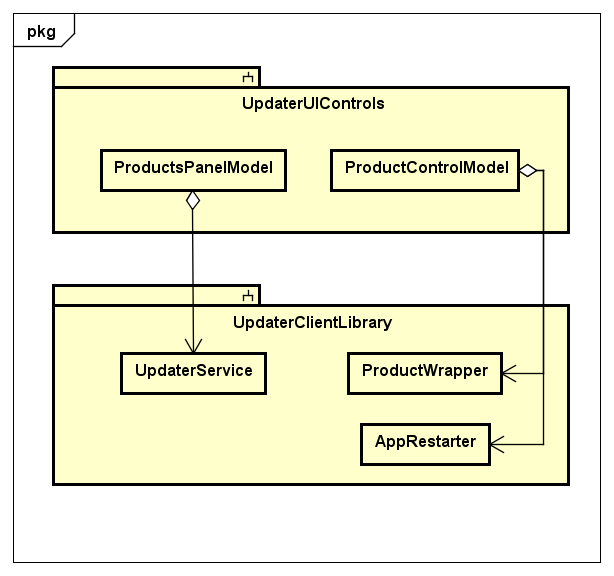
\includegraphics[width=\textwidth]{RelazioniUpdaterUIControls}
				\label{fig:RelazioniUpdaterUIControls}
				\caption{Relazioni componenti di Updater UIControls con le componenti di Client Library}
			\end{figure}
	
\newpage		
		\subsection{Relazioni Updater Client Library}
			\begin{figure}[h]
				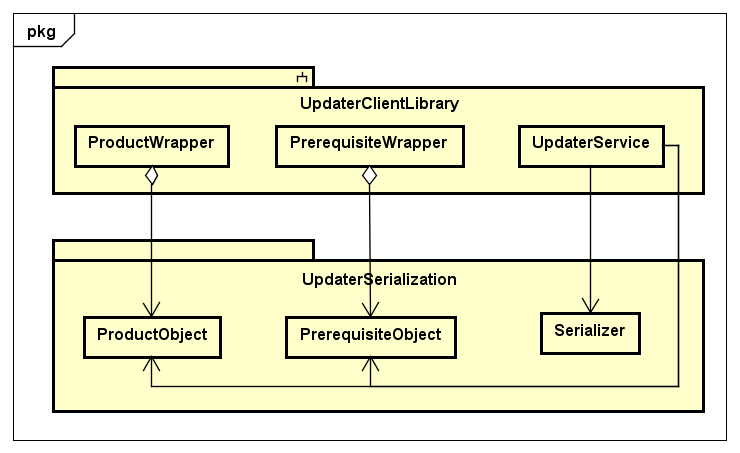
\includegraphics[width=\textwidth]{RelazioniUpdaterClientLibrary}
				\label{fig:RelazioniUpdaterClientLibrary}
				\caption{Relazioni componenti di Updater Client Library con le componenti di Updater Serialization}
			\end{figure}

\newpage			
		\subsection{Relazioni Updater Server}
			\begin{figure}[h]
				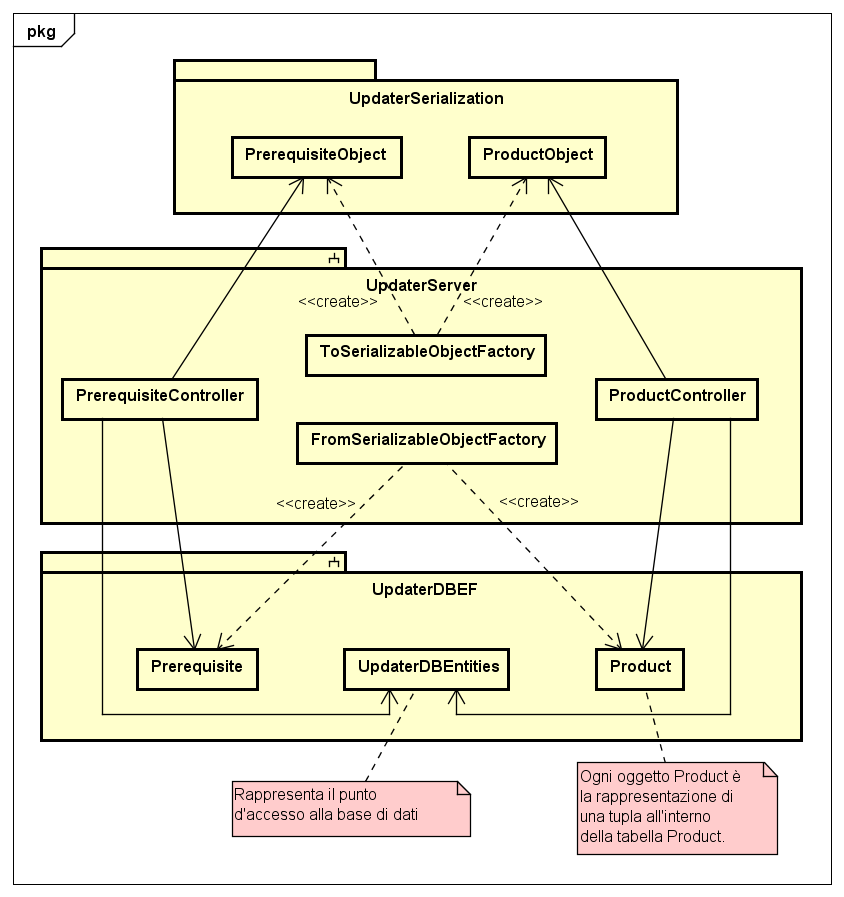
\includegraphics[width=\textwidth]{RelazioniUpdaterServer}
				\label{fig:RelazioniUpdaterServer}
				\caption{Relazioni componenti di Updater Server con le componenti di Updater Serialization e UpdaterEBEF}
			\end{figure}
			
			

\end{document}